\title{Numerical methods, Project 2, on the approximation of functions}
\maketitle
\newpage
\section{Intro}
The algorithms and their plotting, required a large amount of computational power, which my computer lacks. I therefore used markov, NTNU's computational server, giving me the ability to run multiple jupyter notebooks at once, without stressing my own computer. It did not seem like this gave me any substantial improvements in the running time of my algorithms, but the practicality and reliability of markov made it easy to test different parameters for the time consuming gradient descent algorithms.
\newline The creation of every figure is described in the Jupyter notebook.

\section{Problem a)}
The first problem is the foundation of the entire project, namely the implementation of the Lagrange interpolation polynomial. There's multiple ways to do this, each with their own advantages. In the pursuit of an effective and versatile implementation, I implemented the Lagrange polynomial in a way that evaluation in $x$ was just like evaluating a polynomial in $x$. To accomplish this, I used the numpy function ``poly1d'', taking an array of coefficients as input and outputting the relevant polynomial $P$ an object we could evaluate in $x$.
\newline This implementation, LaGrange() in the code, had a few disadvantages. An apparent lack of precision when using more than $20$ nodes and bad synergy with the autograd-package. As a result I decided to write a new implementation, LaGrange2() in the code, recalculating the interpolated polynomial for every value of $x$ we are evaluating. Of course the interpolated polynomial only changes when changing the nodes, but now we never actually calculate the polynomial coefficients by itself, but rather their values for one unique $x$ at a time.
\newline The problem description asks for a Python function taking interpolating nodes $\{(x_i)_{i\in\N}\}$ and the corresponding values $\{f(x_i)_{i\in\N}\}$ as inputs along with the value of $x$ we are evaluating in. My implementation takes the function, $f$, which we want to approximate as input, technically assuming it's known and thereby in conflict with the problem description, but our Python function only ever evaluate $f$ in the nodes $x_i$, which in practice should make my implementation equivalent to only knowing the function values in the nodes as there would be little to no computational difference between my implementation and simply evaluating the function in the nodes beforehand.
\newline Figure 1 shows a plot of the Runge function
  $$ f(x)=\frac{1}{x^2+1} \quad,\quad x\in[-5,5] \quad,\quad n=10$$
with both equidistant nodes and Chebyshev nodes.
\begin{figure}\label{Figure 1}
  \begin{center}
  \caption{Plot of the Runge function}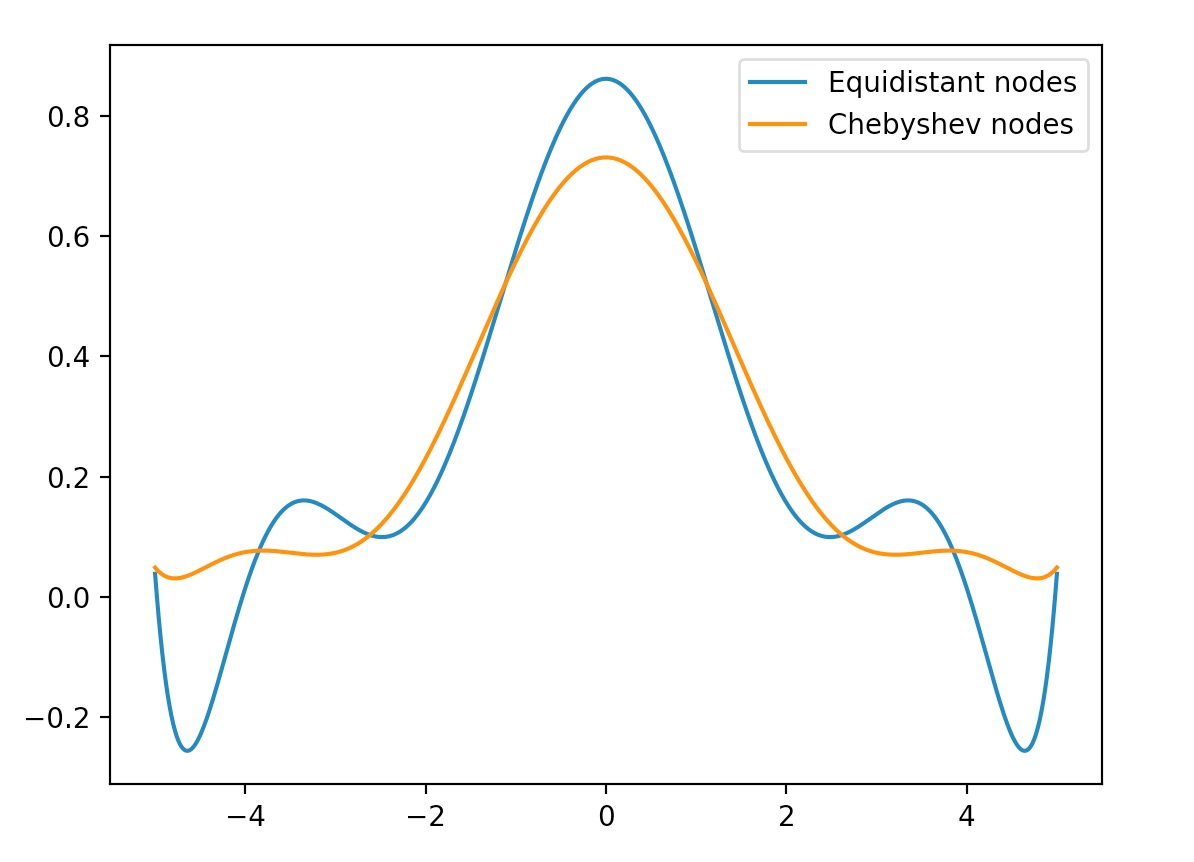
\includegraphics[width=0.30\paperwidth]{vaar2020/numerical_methods/rungeplot}
\end{center}
\end{figure}
This plot is a great demonstration of the Runge phenomenom (Suli, Mayers, 2003., p. 186)\ref{NumAnal}, and with an increase in the degree of our interpolation polynomial we would see an exponential increase in the maximum error $max_{x\in[-5,5]}|f(x)-p_n(x)|$.

\section{Problem b)}
For this problem, we are asked to study to different functions,  $f$ and $g$:
$$ f(x)=\cos(2\pi x), x\in[0,1]$$
$$ g(x)=e^{3x}\sin(2x), x\in [0, \pi/4]$$
To judge the quality of our Lagrange polynomials, we need to do compute the approximated error in different norms. We look at the following approximations for $||f-p_n||$ in the max-norm and $2$-norm, respectively:
$$ ||f-p_n||_{\infty} \approx max_{\eta_0, \dots, \eta_N}|f(\eta_i)-p_n(\eta_i)|, \qquad ||f-p_n||_{2}\approx \frac{\sqrt{b-a}}{\sqrt{N}}\left(\sum_{i=0}^{N}(f(\eta_i)-p_n(\eta_i))^2\right)^{\frac{1}{2}},$$
where $N=100n$ and denotes the number of known points, $\eta_i$, on the curve, with $x_0=\eta_0<\eta_1<\dots \eta_N=x_n$.
\newline From theorem $6.2$ (Suli, Mayers, 2003., p. 183)\ref{NumAnal} in the book, we have a theoretical error bound for the interpolation error:
$$ \left|f(x)-p_{n}(x)\right| \leq \frac{M_{n+1}}{(n+1) !}\left|\pi_{n+1}(x)\right| ,$$
where $\pi_{n+1}(x)=\left(x-x_{0}\right) \ldots\left(x-x_{n}\right)$ and $M_{n+1}=\max _{\zeta \in[a, b]}\left|f^{(n+1)}(\zeta)\right|$. For $f(x)=\cos(2\pi x)$, observe that
$$ \frac{\partial^n f(x)}{\partial x^n} = (2\pi)^n\cos(\frac{1}{2}\pi(n+4x)) \Rightarrow \frac{\partial^{n+1} f(x)}{\partial x^{n+1}} = (2\pi)^{n+1}\cos(\frac{1}{2}\pi(n+4x+1)), n\in \Z, n\geq 0.$$
Indeed $\max _{\zeta \in[a, b]}\left|f^{(n+1)}(\zeta)\right|=(2\pi)^{n+1}$. Since we are approximating $f(x)$ on $[0,1]$, every term in $\pi_{n+1}(x)$ will be between $-1$ and $1$, making $|\pi_{n+1}(x)|<1$. Hence,
$$ \left|f(x)-p_{n}(x)\right| \leq \frac{(2\pi)^{n+1}}{(n+1)!}, $$
which is our theoretical error bound.

\begin{figure}[H]
    \centering
    \begin{minipage}{0.45\textwidth}
        \centering
        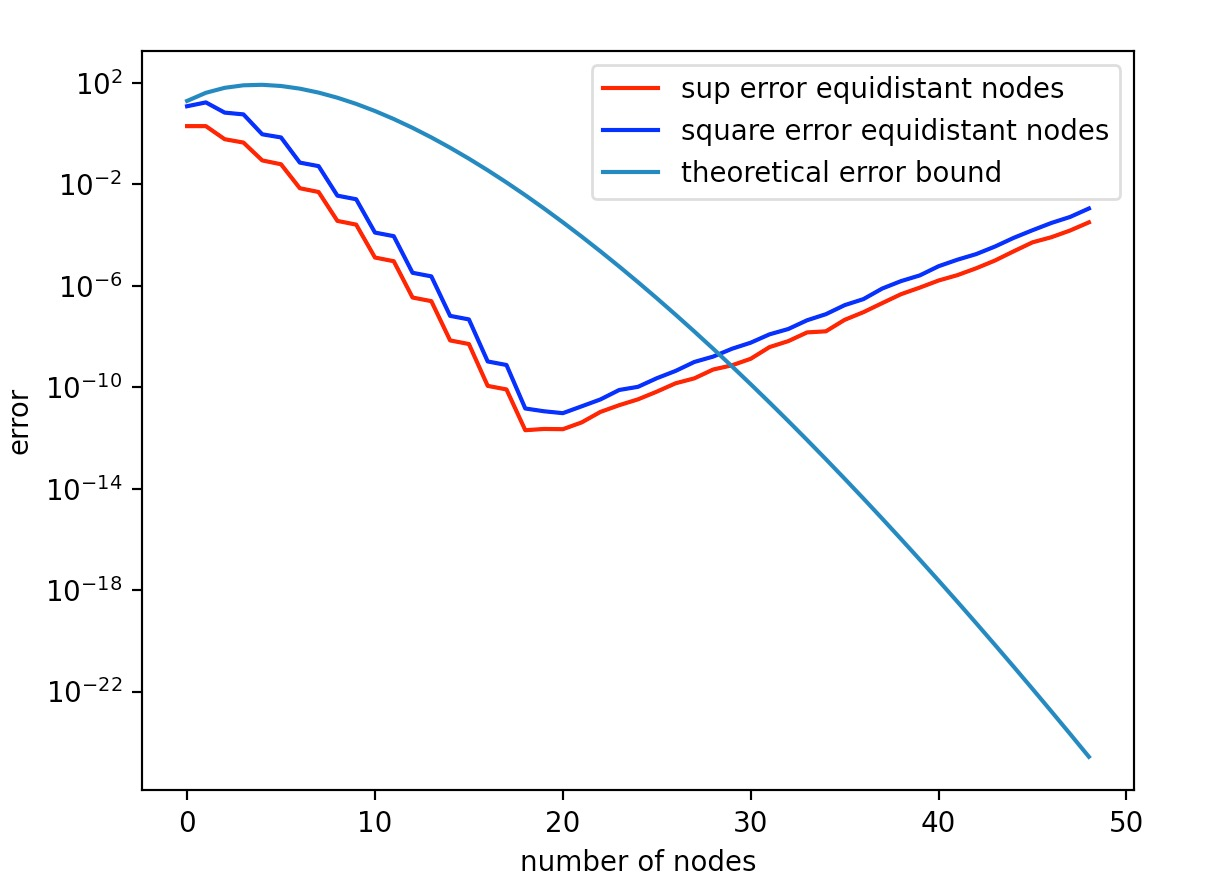
\includegraphics[width=1.05\textwidth]{vaar2020/numerical_methods/errors_vs_nodes_F_equi} % first figure itself
        \caption{$f(x)$ with equidistant nodes}
    \end{minipage}\hfill
    \begin{minipage}{0.45\textwidth}
        \centering
        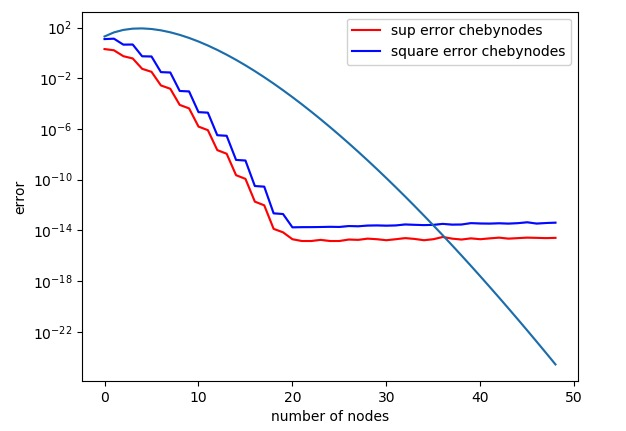
\includegraphics[width=1.05\textwidth]{vaar2020/numerical_methods/errors_vs_n_F_cheby} % second figure itself
        \caption{$f(x)$ with Chebyshev nodes}
    \end{minipage}
\end{figure}
\begin{figure}[H]
    \centering
    \begin{minipage}{0.45\textwidth}
        \centering
        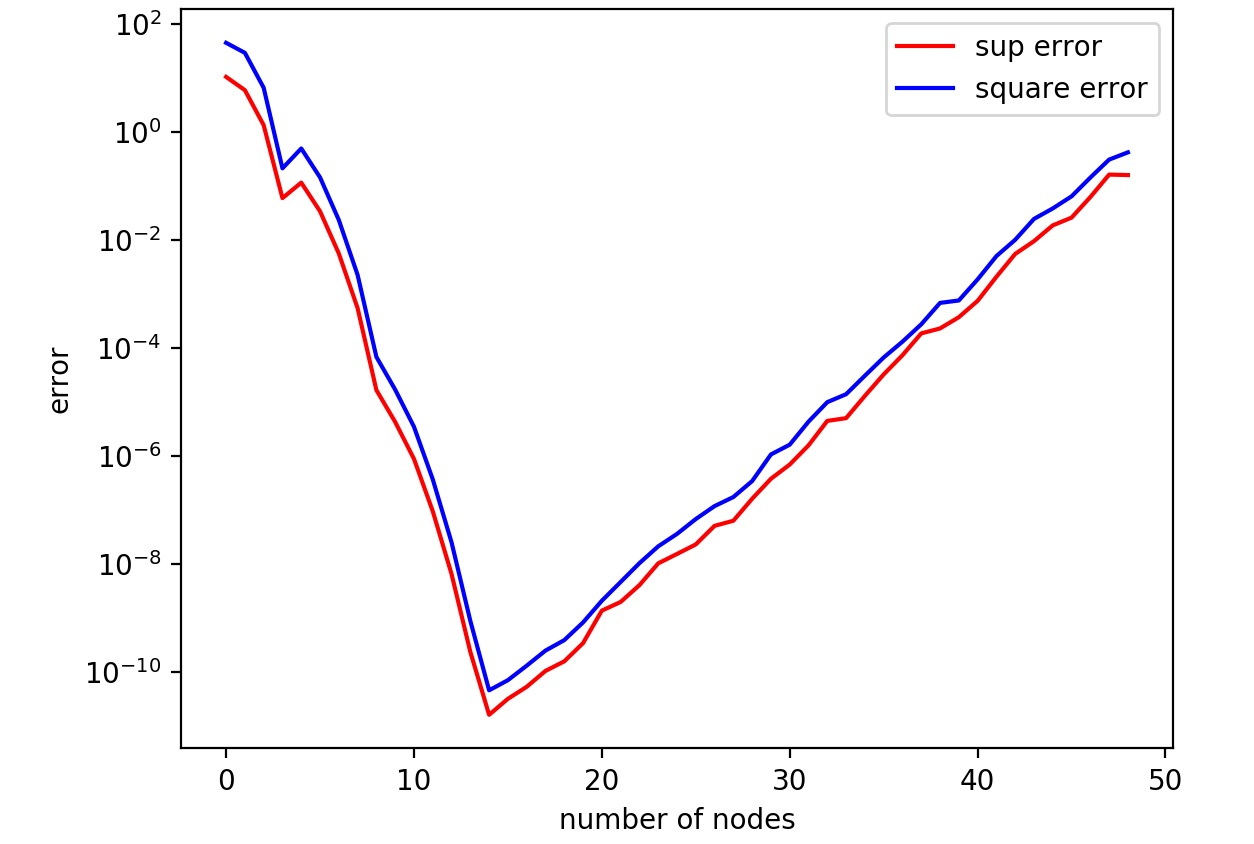
\includegraphics[width=1.05\textwidth]{vaar2020/numerical_methods/errors_vs_nodes_G-equi} % first figure itself
        \caption{$g(x)$ with equidistant nodes}
    \end{minipage}\hfill
    \begin{minipage}{0.45\textwidth}
        \centering
        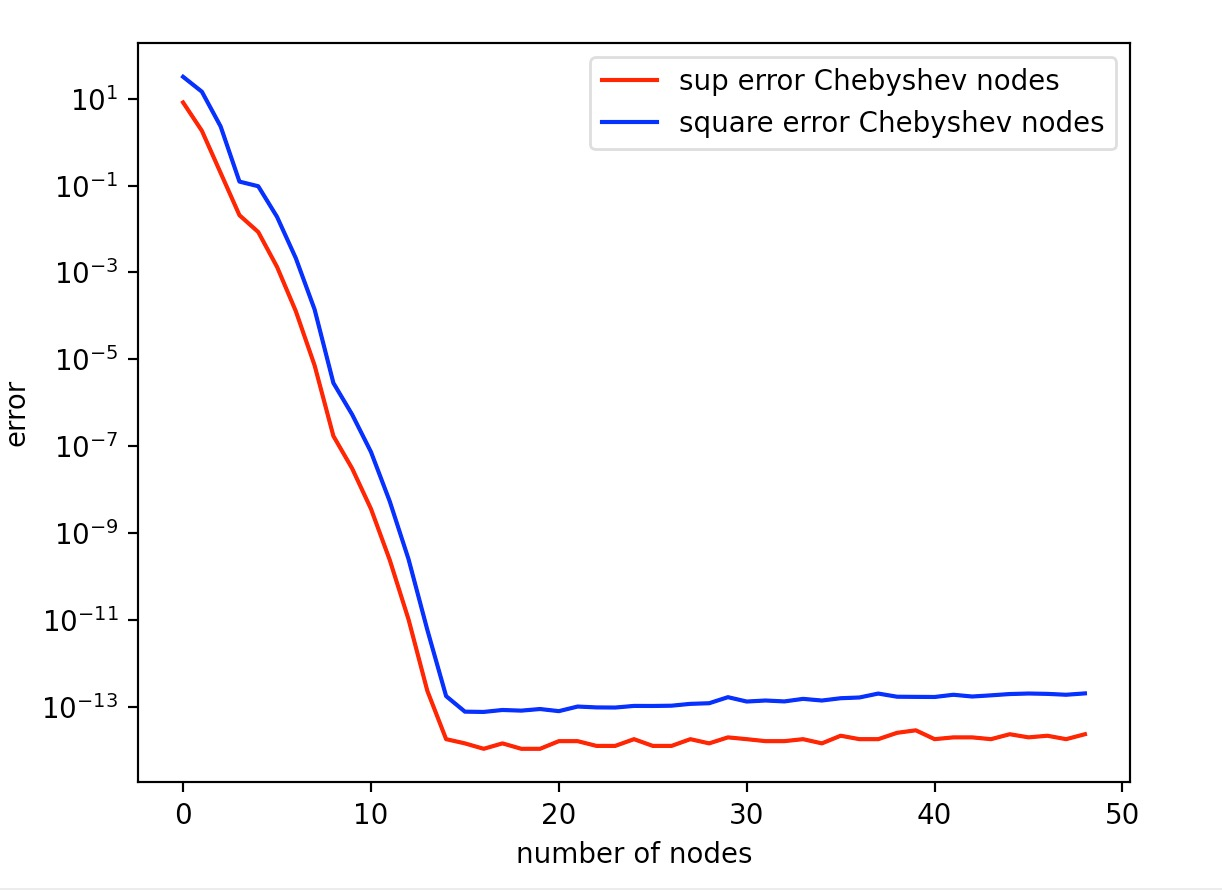
\includegraphics[width=1.05\textwidth]{vaar2020/numerical_methods/error_vs_nodes_G_cheby} % second figure itself
        \caption{$g(x)$ with Chebyshev nodes}
    \end{minipage}
\end{figure}
The figures display the difference between equidistant and Chebyshev nodes. For these two functions, the Runge phenomenom should not appear, but nevertheless something interesting happens when $n>20$. The approximated errors start eclipsing the theoretical error bound when using equidistant nodes for both functions. I suspect the cause of this behaviour originates from some form of propagation of error related to floating point precision in numpy. For Chebyshev nodes the approximated error flats out at $10^{-14}$ presumably because of machine precision, which is around $2*10^{-16}$ for numpy floating numbers.

\section{Problem c)}
This problem asks us to subdivide the interval we are interpolating on into $K$ subintervals, and then do Lagrange interpolation separately on each subinterval.
\newline The Python function, piecewiseLaGrange(), subdivides the interval $[a,b]$ into $K$ smaller intervals, and then performs LaGrange interpolation on those subintervals by calling the function implemented in a).
\begin{figure}[H]
    \centering
    \begin{minipage}{0.45\textwidth}
        \centering
        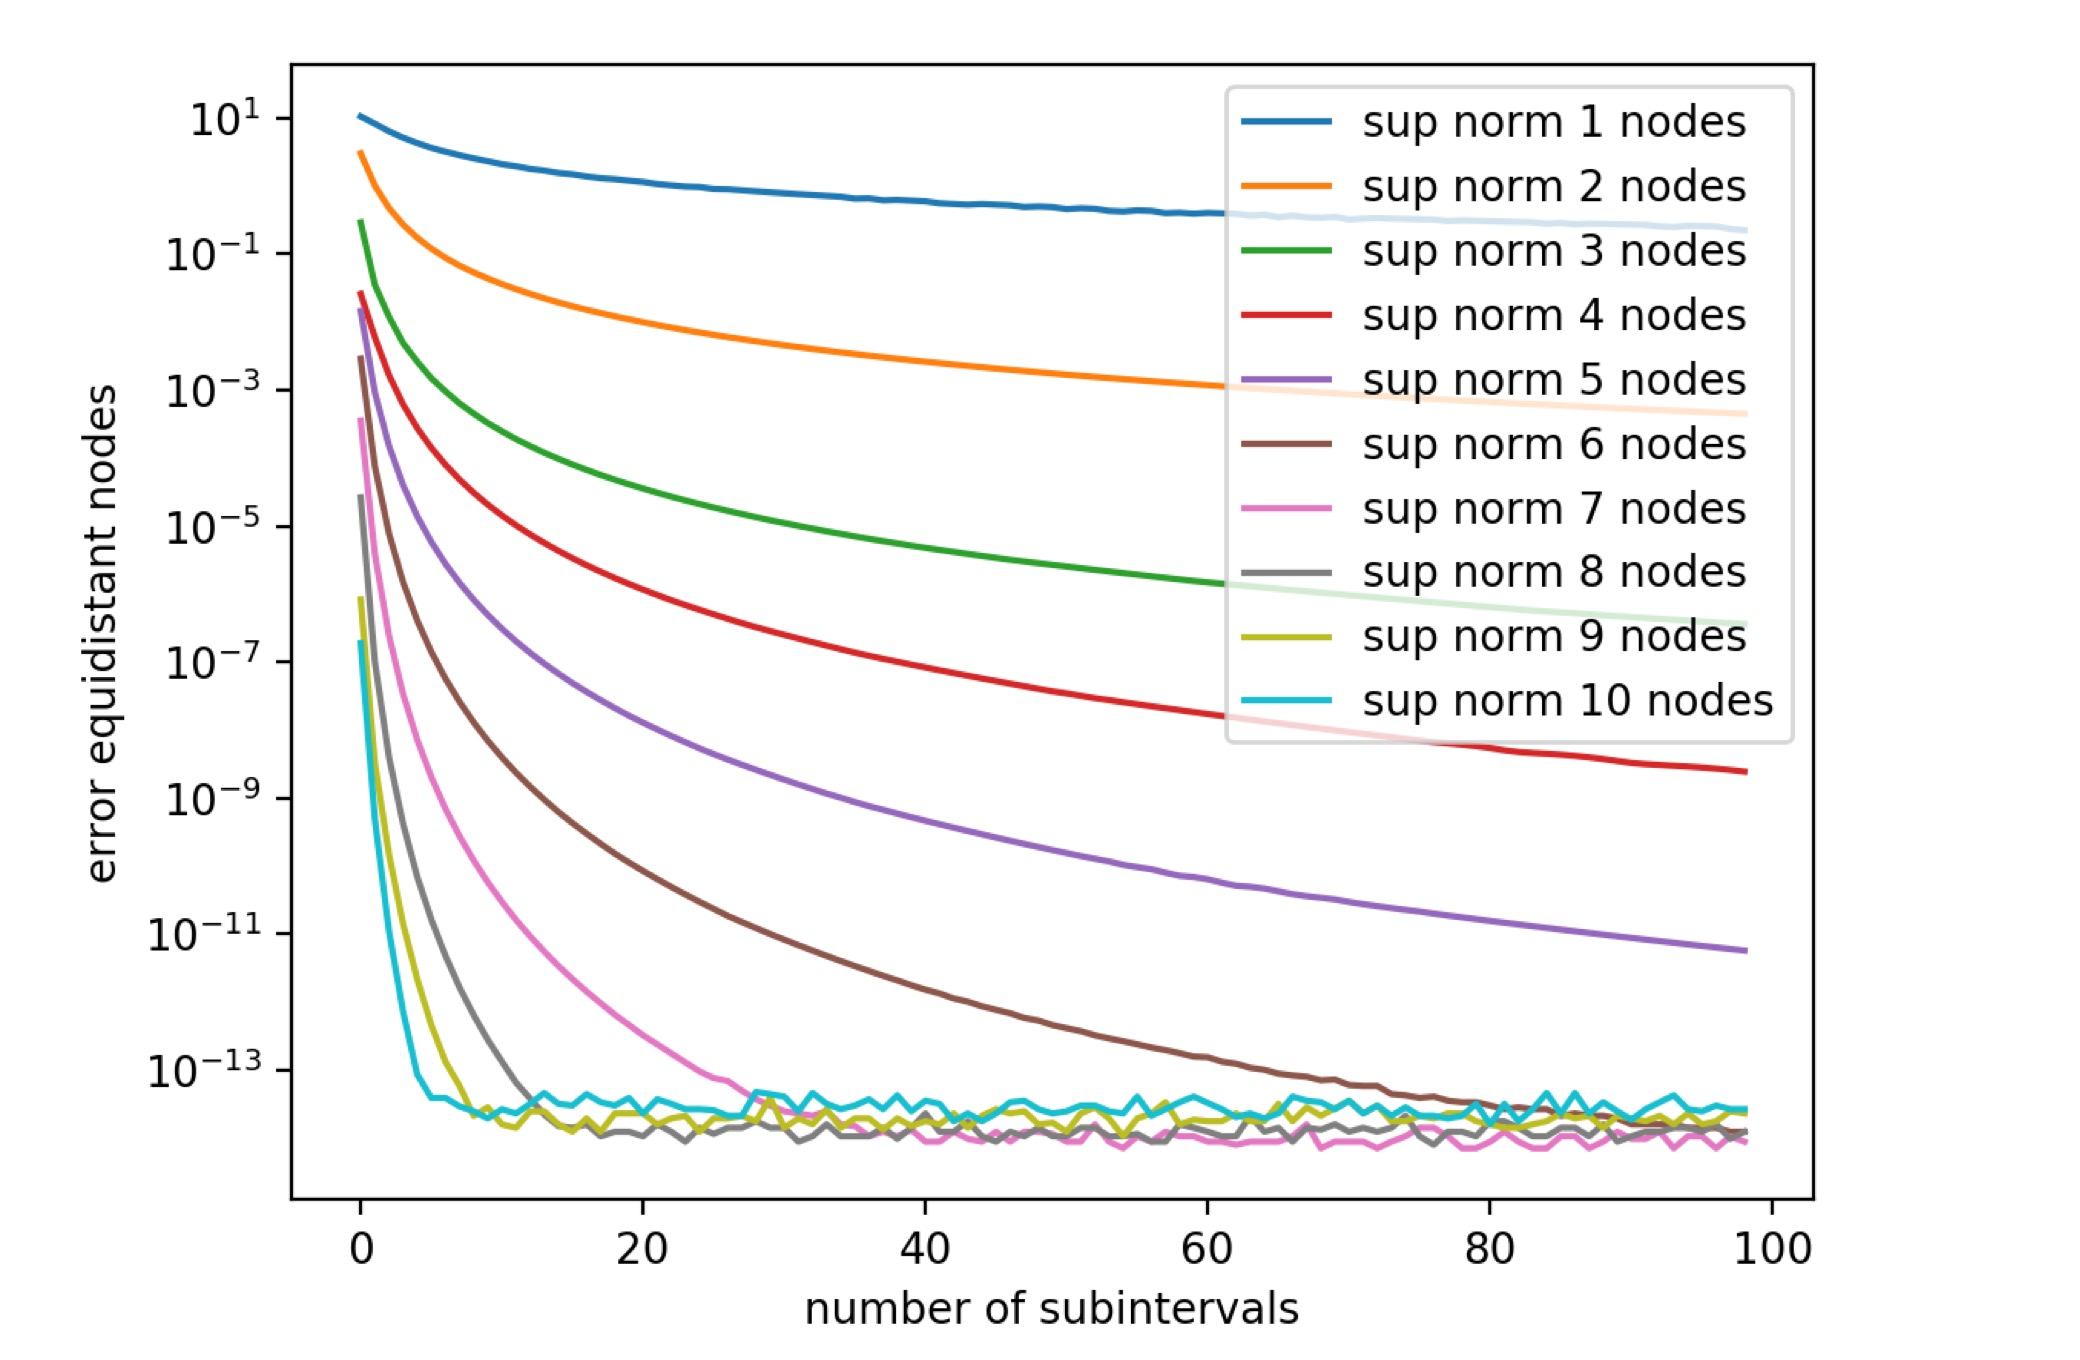
\includegraphics[width=1.05\textwidth]{vaar2020/numerical_methods/Piecewise_Lagrange_G_equidist_2} % first figure itself
        \caption{$g(x)$ with equidistant nodes}
    \end{minipage}\hfill
    \begin{minipage}{0.45\textwidth}
        \centering
        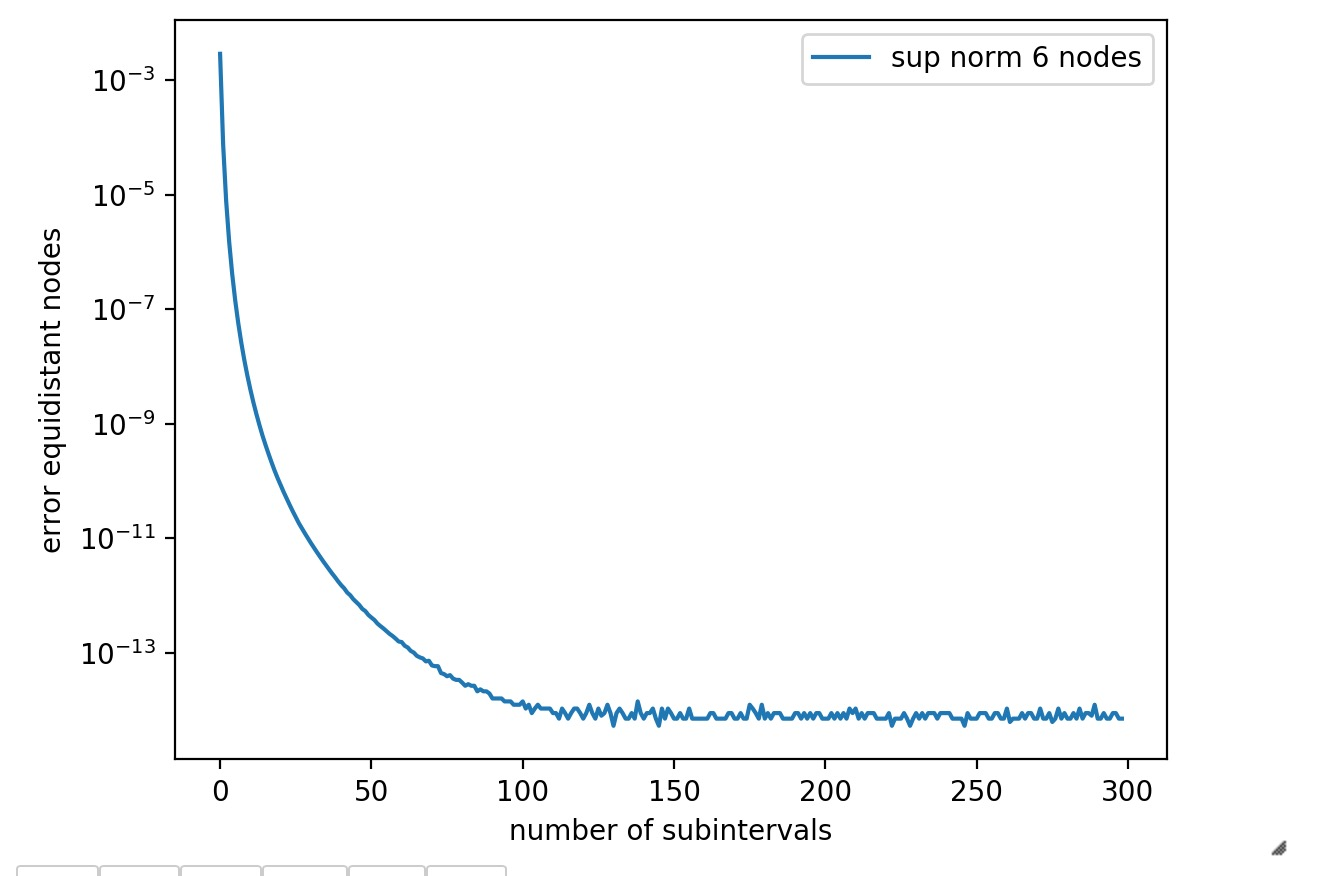
\includegraphics[width=1.05\textwidth]{vaar2020/numerical_methods/PWL_G_3} % second figure itself
        \caption{$g(x)$ with equidistant nodes}
    \end{minipage}
\end{figure}
It is apparent from the figures that the error goes to zero as the number of subintervals $K$ goes to $\infty$ (or at least to $10^{-14}$ due to machine precision). Observe also that the piecewise interpolation does not seem to give the same problem for equidistant nodes as in the previous problem, perhaps because we avoid using a large number of nodes.
\newline Looking at the computational cost of our iplementation of piecewise Lagrange interpolation, we see that our while loop terminates when $i >=b$ after $n$ iterations.
This occurs when $n = k$, so it is at worst $O(K)$
The for loop is at best only looking at the first element $X$
and in the worst case looking at every element in X.
So best case is $O(1)$ and worst case is $O(n)$.
Producing equidist nodes is $O(n)$, and our eval function is $O(1)$
Finally, our Lagrange2's for loop is $O(n^2)$ and the sum is $O(n)$
As such we find that $O(K + n^2)$ is the dominating degree in both the best and worst case.
Noting that if $K >> n$, then it evaluates to $O(K)$.

\section{Problem d)}
This problem asks us to use a gradient descent algorithm optimize the nodes we use for interpolation. My implementation is the same as the one in the appendix, and I only use gradient descent with backtracking throughout all my experiments.
\newline Gradient descent is an algorithm used to minimize some function by iteratively moving in the direction of the steepest descent. The function we want to minimize is the cost function:
$$ \mathcal{C}(X)=\frac{b-a}{N}\sum_{k=0}^{N}\left(f(\xi_k)-p_n(\xi_k)\right)^2 ,\quad p_{n}(\xi)=\sum_{i=0}^{n} \ell_{i}(\xi) f\left(x_{i}\right), \quad \ell_{i}(\xi)=\prod_{j=0, j \neq i}^{n} \frac{\xi-x_{j}}{x_{i}-x_{j}}$$
$p_n$ is the Lagrange interpolation polynomial as used earlier. My implementation uses the Python package Autograd for automatic differentiation of our cost function. Therefore we must implement the cost function as a function of only one variable, namely $X$, our interpolation nodes. The implemented function for $\mathcal{C}(X)$ still needs access to $f(\eta_i)$ for all $\eta_i\notin X$, and to accomplish this we once again assume $f$ is known. There is a function p() in the code, which stores and gives $\mathcal{C}(X)$ access to all the necessary variables.
\newline There are three different parameters affecting gradient descent's convergence. There's the step size $L$ and two hyperparameters hyp1 and hyp2. Through numerous experimenting with different parameters, I found $L=100, \quad hyp1=2, \quad hyp2=0.9$ to work fine. I always initialize with equidistant nodes. To display the effect of gradient descent I plot $\mathcal{C}(X)$ versus the number of iterations in the ``outer loop'' of the algorithm.
\begin{figure}[H]
    \centering
    \begin{minipage}{0.45\textwidth}
        \centering
        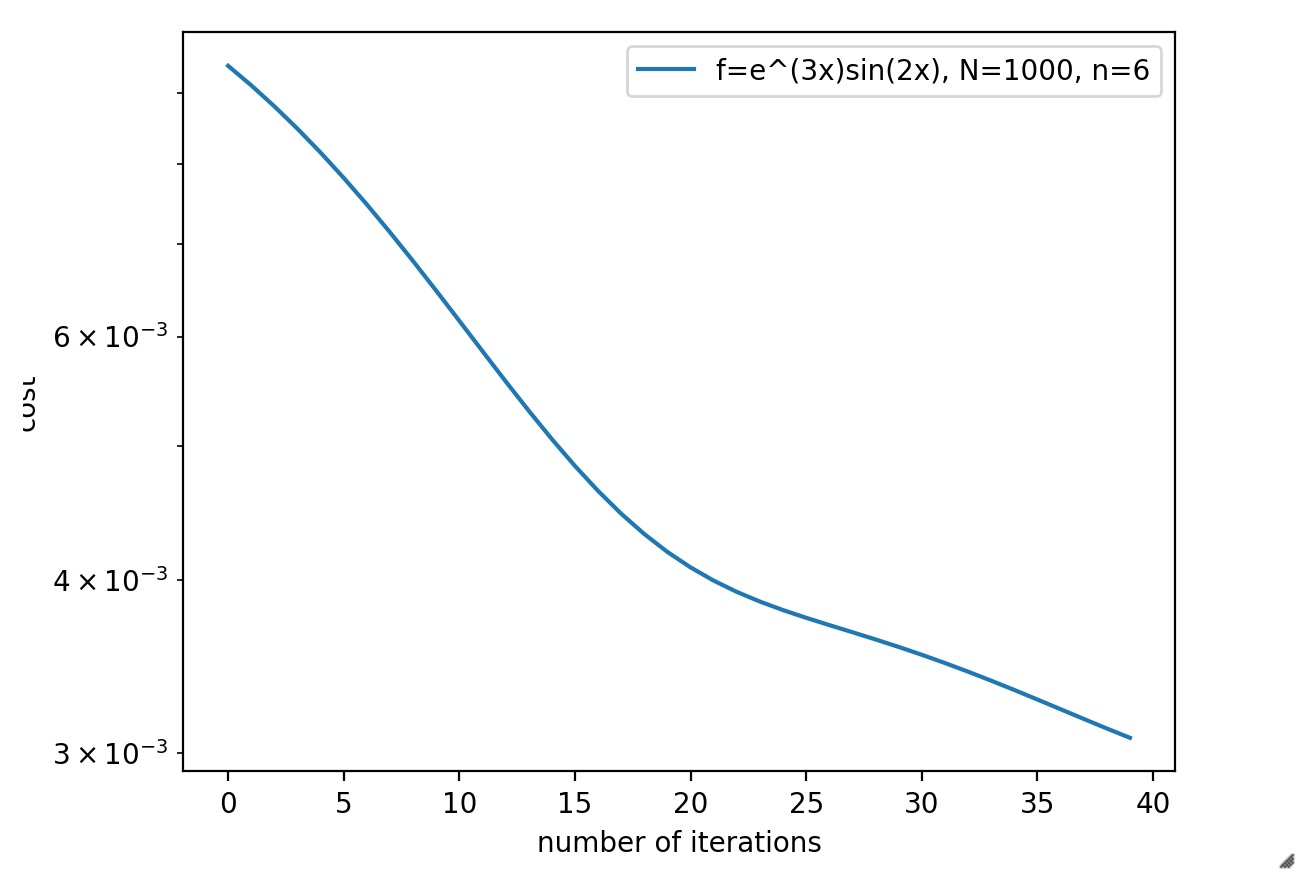
\includegraphics[width=1.05\textwidth]{vaar2020/numerical_methods/cost_vs_iterations_G} % first figure itself
        \caption{$g(x)$}
    \end{minipage}\hfill
    \begin{minipage}{0.45\textwidth}
        \centering
        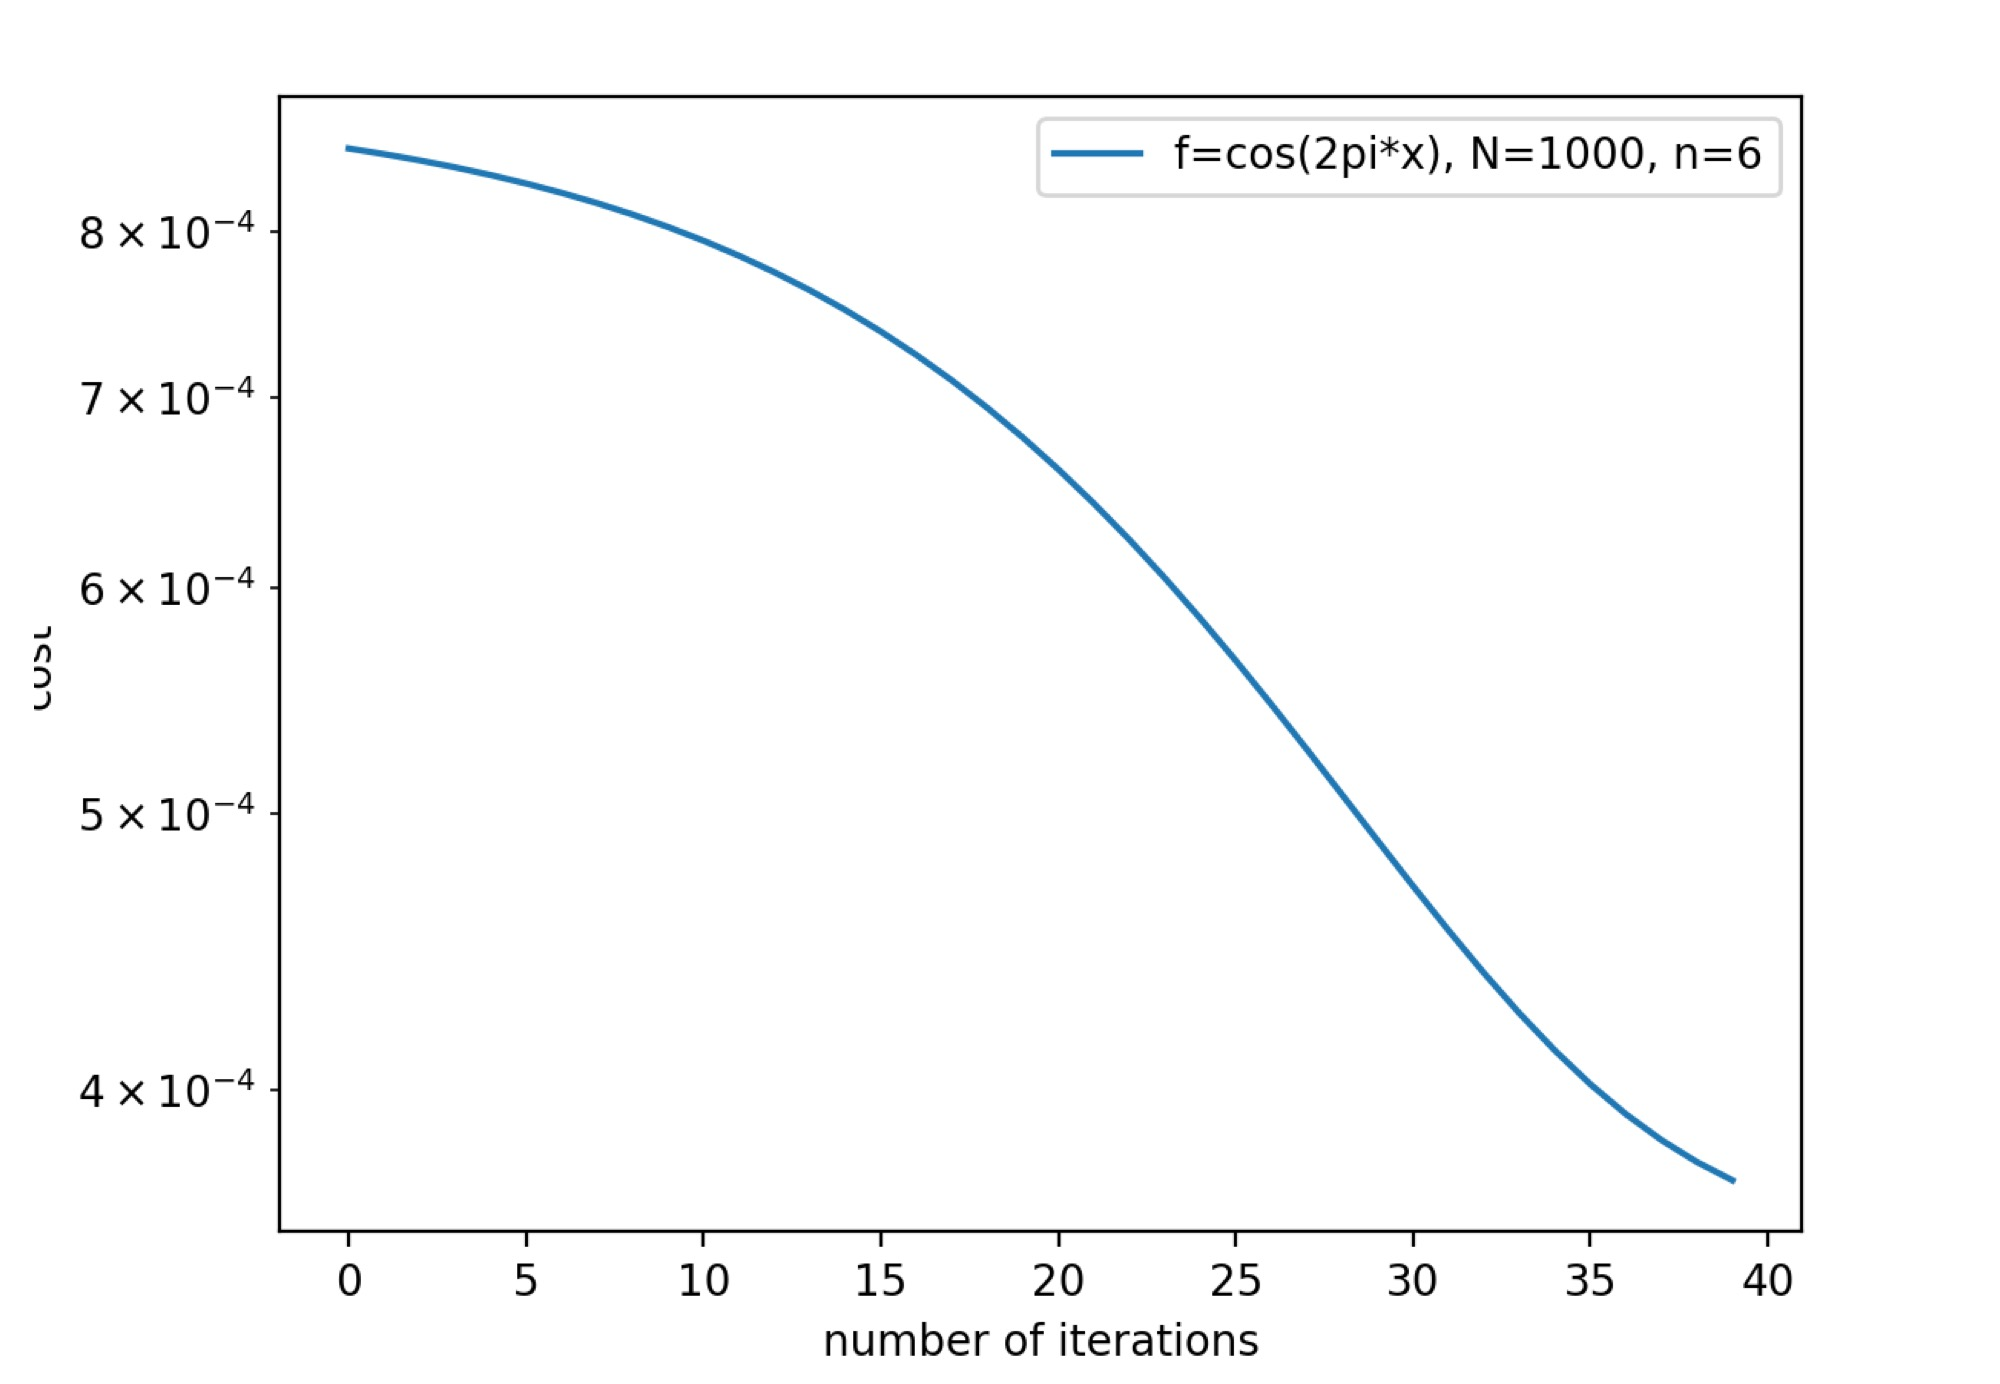
\includegraphics[width=1.05\textwidth]{vaar2020/numerical_methods/cost_vs_iterations_F} % second figure itself
        \caption{$f(x)$}
    \end{minipage}
\end{figure}
As desired, the cost decreases as the number of iterations increases. The inherent relationship between the cost function and the approximated square error implies that the square error would decrease with the increase of iterations. Reusing the setup used in figure 2 and 3, I have plotted the square error for $f(x)$ with $n\in[1,10]$, and equidistant and Chebyshev nodes alongside the nodes aqquired from $100$ iterations of gradient descent:
\begin{figure}[H]
  \begin{center}
  \caption{Square error vs number of nodes}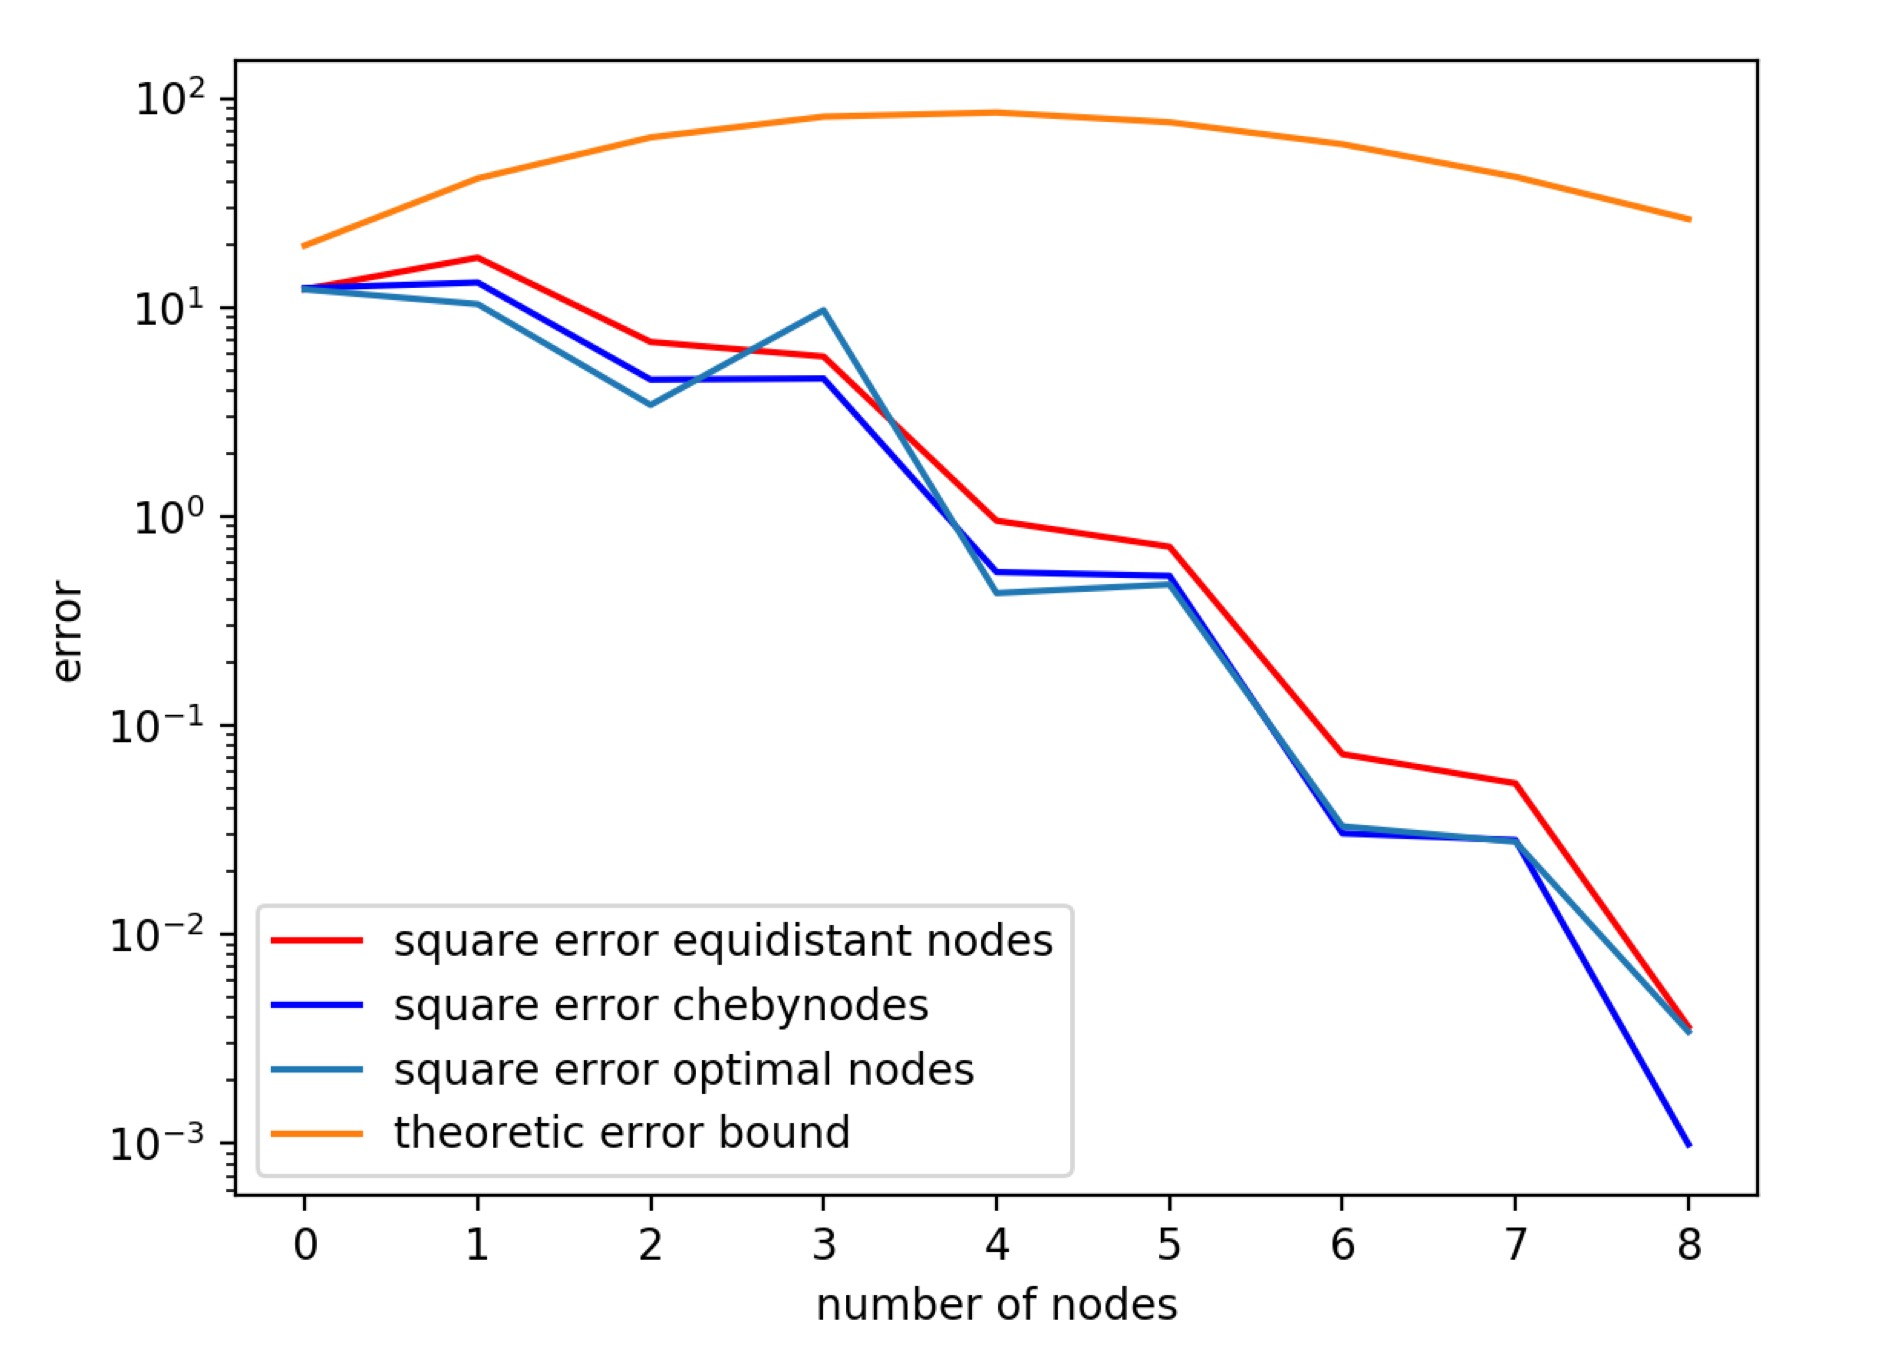
\includegraphics[width=0.30\paperwidth]{vaar2020/numerical_methods/error_vs_nodes_F_100_iters}
\end{center}
\end{figure}
From the graph it is apparent that Chebyshev nodes already fits the function $f(x)=\cos(2\pi x)$ quite nicely as the nodes from gradient descent only seems marginally better for some $n$ and surprisingly worse for other $n$.
\newline In theory, the gradient descent algorithm should be able to optimize the nodes well enough to beat Chebyshev nodes. More experimentation with different parameters and a higher number of iterations would probably accomplish this. Thus it would pay off to invest more time and energy into writing better and more effective code -- I am certainly no expert -- or even consider calculating the gradient by hand or through other methods than autograd, sacrificing convenience for speed.

\section{Problem e)}
This problem asks us to swap the interpolation polynomial for a  radial basis function to approximate $f$. We will use the following approximation:
$$ f(x) \approx \tilde{f}(x)=\sum_{i=0}^{n} w_{i} \phi\left(\left|x-x_{i}\right|\right), \quad \phi(r)=\exp \left(-(\varepsilon r)^{2}\right)$$
with
$$\tilde{f}\left(x_{i}\right)=f\left(x_{i}\right), \quad i=0, \ldots, n,$$
with values $\vct{w}=[w_0, \dots, w_n]^T$ the solution of the linear system $M \mathbf{w}=\mathbf{f}$, where $\mathbf{f}:=\left[f\left(x_{0}\right), \ldots, f\left(x_{n}\right)\right]^{T}$, and $M$ is the $(n+1\times(n+1))$ matrix given by
$$M_{i, j}:=\phi\left(\left|x_{i}-x_{j}\right|\right)$$
making the weight $\vct{w}$ a function of $X$.
\newline The cost function stays the same as before, but with the radial basis function instead of the interpolated polynomial. To ensure that the gradient descent algorithm optimizes over both the nodes X and the shape parameter e, we make the cost function take the array $[x_0, \dots, x_n, \varepsilon]$ as input.
$$\mathcal{C}([X, \varepsilon]):=\frac{b-a}{N} \sum_{k=0}^{N}\left(f\left(\xi_{k}\right)-\tilde{f}\left(\xi_{k}\right)\right)^{2}, \quad \tilde{f}(\xi)=
\sum_{i=0}^{n} w_{i} \phi\left(\left|\xi-x_{i}\right|\right), \quad \mathbf{w}=M^{-1} \mathbf{f}$$
We introduce one more function for approximation:
$$ h(x)=\frac{3}{4}\left(e^{-(9 x-2)^{2} / 4}+e^{-(9 x+1)^{2} / 49}\right)+\frac{1}{2} e^{-(9 x-7)^{2} / 4}-\frac{1}{10} e^{-(9 x-4)^{2}}$$
We plot cost against the number of iterations to show that this implementation is proper.
\begin{figure}[H]
    \centering
    \begin{minipage}{0.45\textwidth}
        \centering
        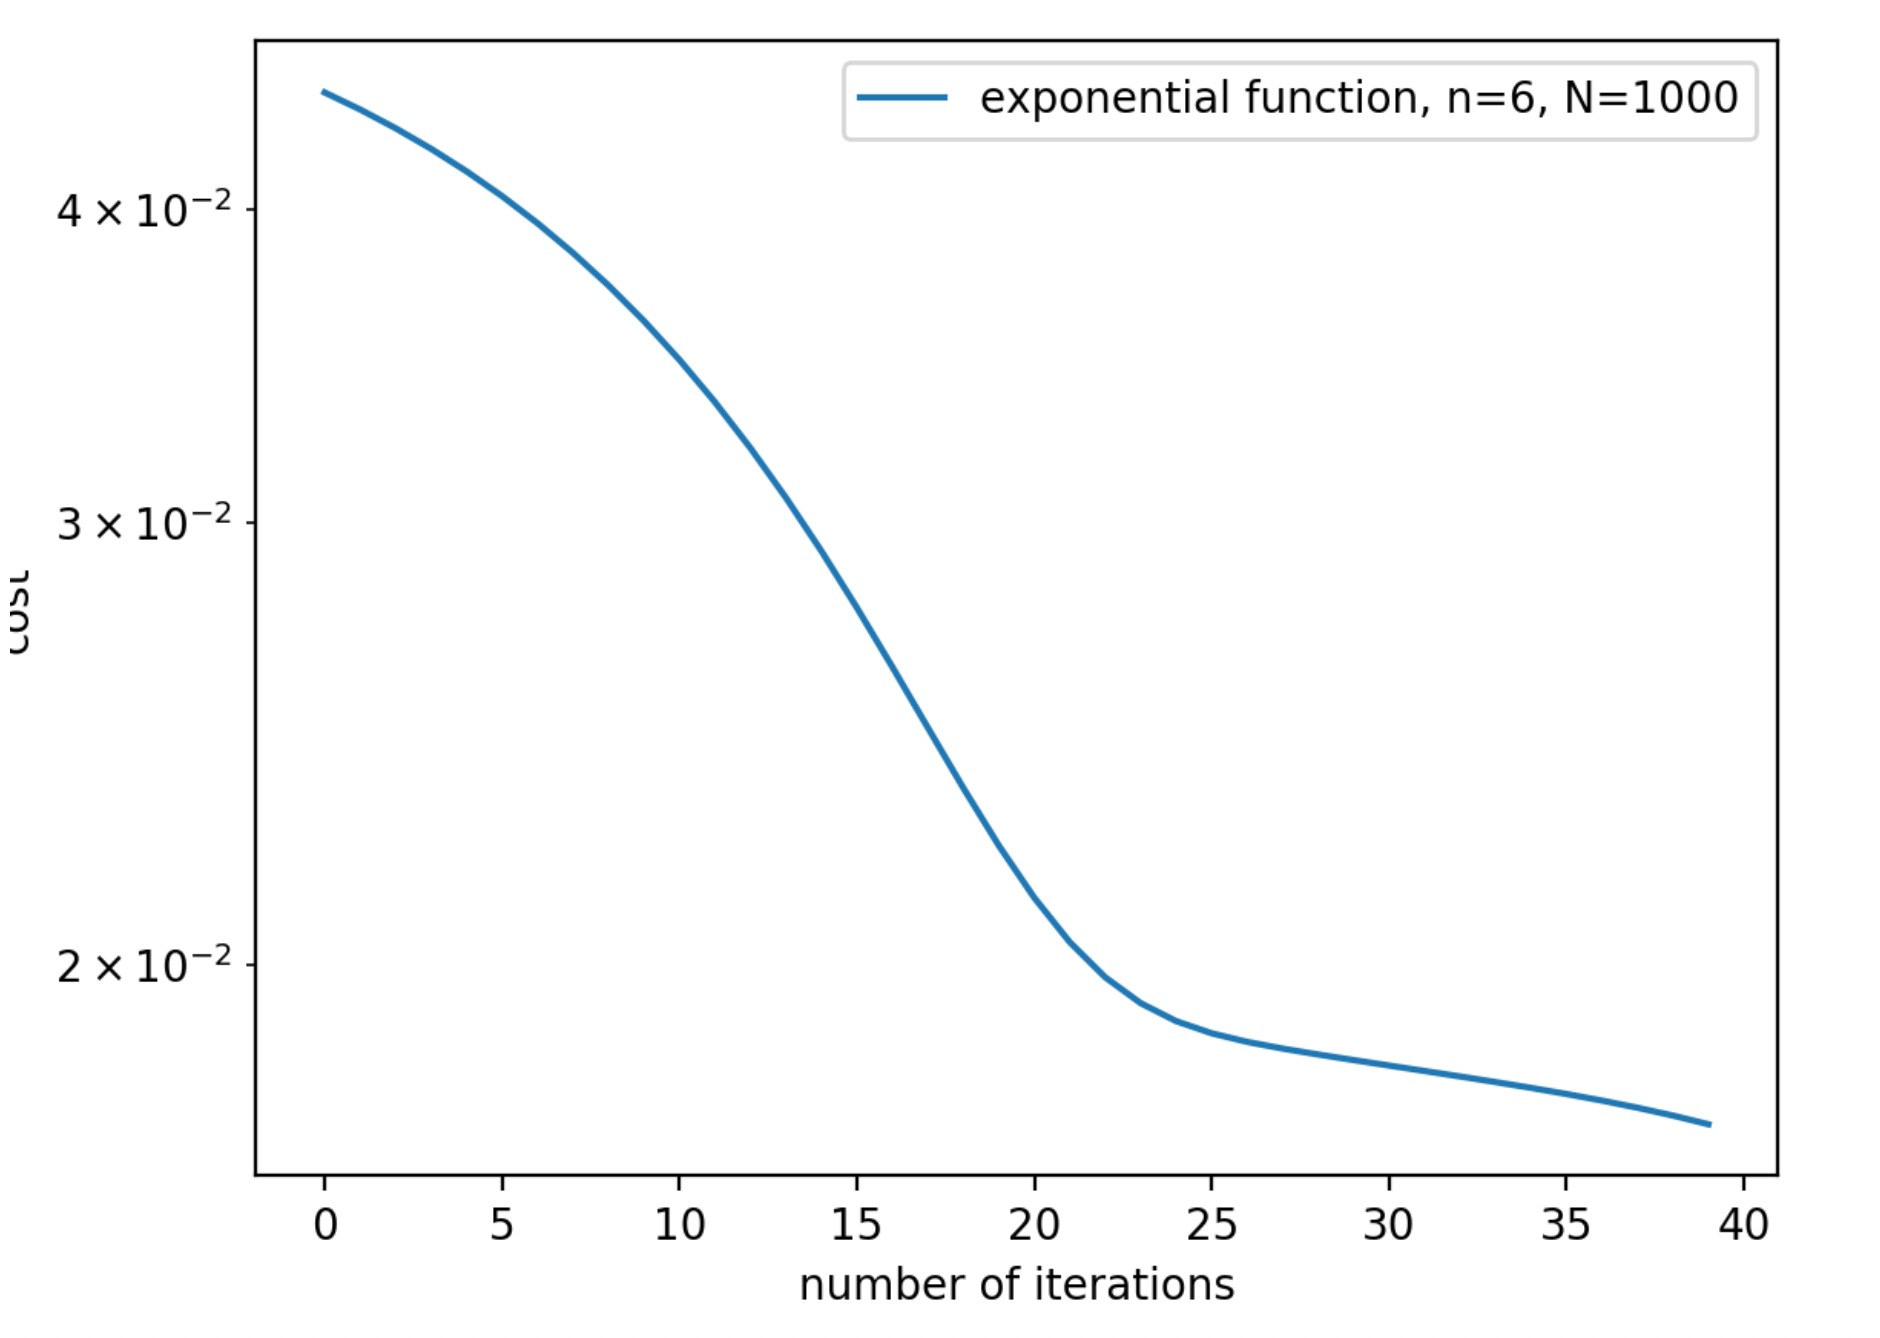
\includegraphics[width=1.05\textwidth]{vaar2020/numerical_methods/cost_vs_iterations_exp} % first figure itself
        \caption{$h(x)$ on $[-1,1]$}
    \end{minipage}\hfill
    \begin{minipage}{0.45\textwidth}
        \centering
        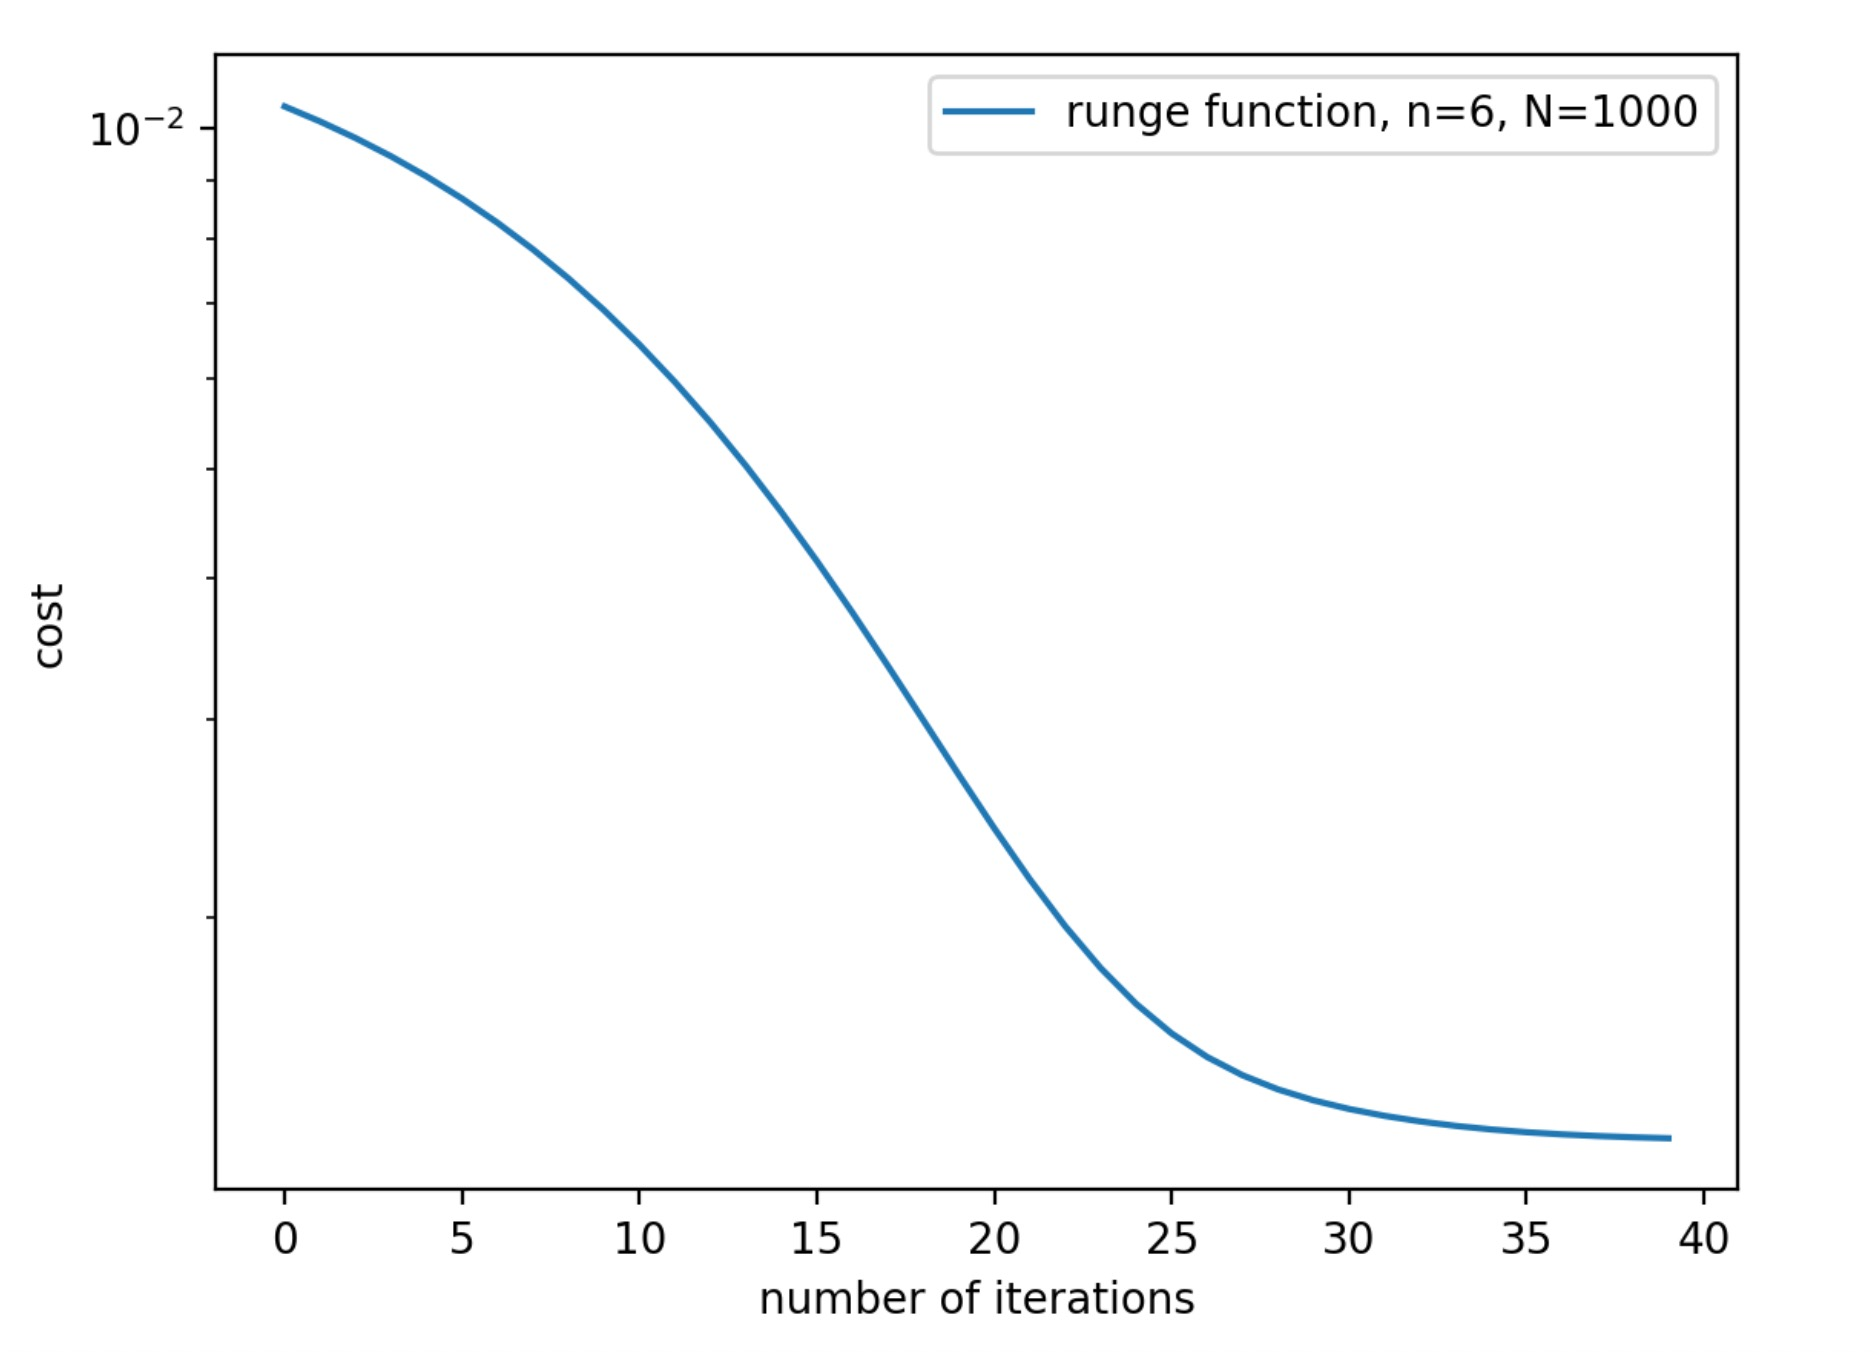
\includegraphics[width=1.05\textwidth]{vaar2020/numerical_methods/cost_vs_iterations_runge} % second figure itself
        \caption{The Runge function on $[-1,1]$}
    \end{minipage}
\end{figure}
Comparing this plot to the one done on $f$ and $g$ in the preceding section, we see that the cost is roughly two orders of magnitude bigger for the same number of iterations this time.
Implying, as noted in the project, that this is a more difficult optimization problem. On the other hand, plotting the square error against the number of nodes for equidistant -, Chebyshev - and gradient descent optimized nodes reveals that the optimized nodes are much better. Perhaps hinting that equidistant- and Chebyshev nodes are bad initial guesses for these functions. I will remark that the theory for Chebyshev nodes does not apply in the same sense for radial basis functions as it does for polynomial interpolation. Yet, I decided to include it as a curiosity.
\begin{figure}[H]
    \centering
    \begin{minipage}{0.45\textwidth}
        \centering
        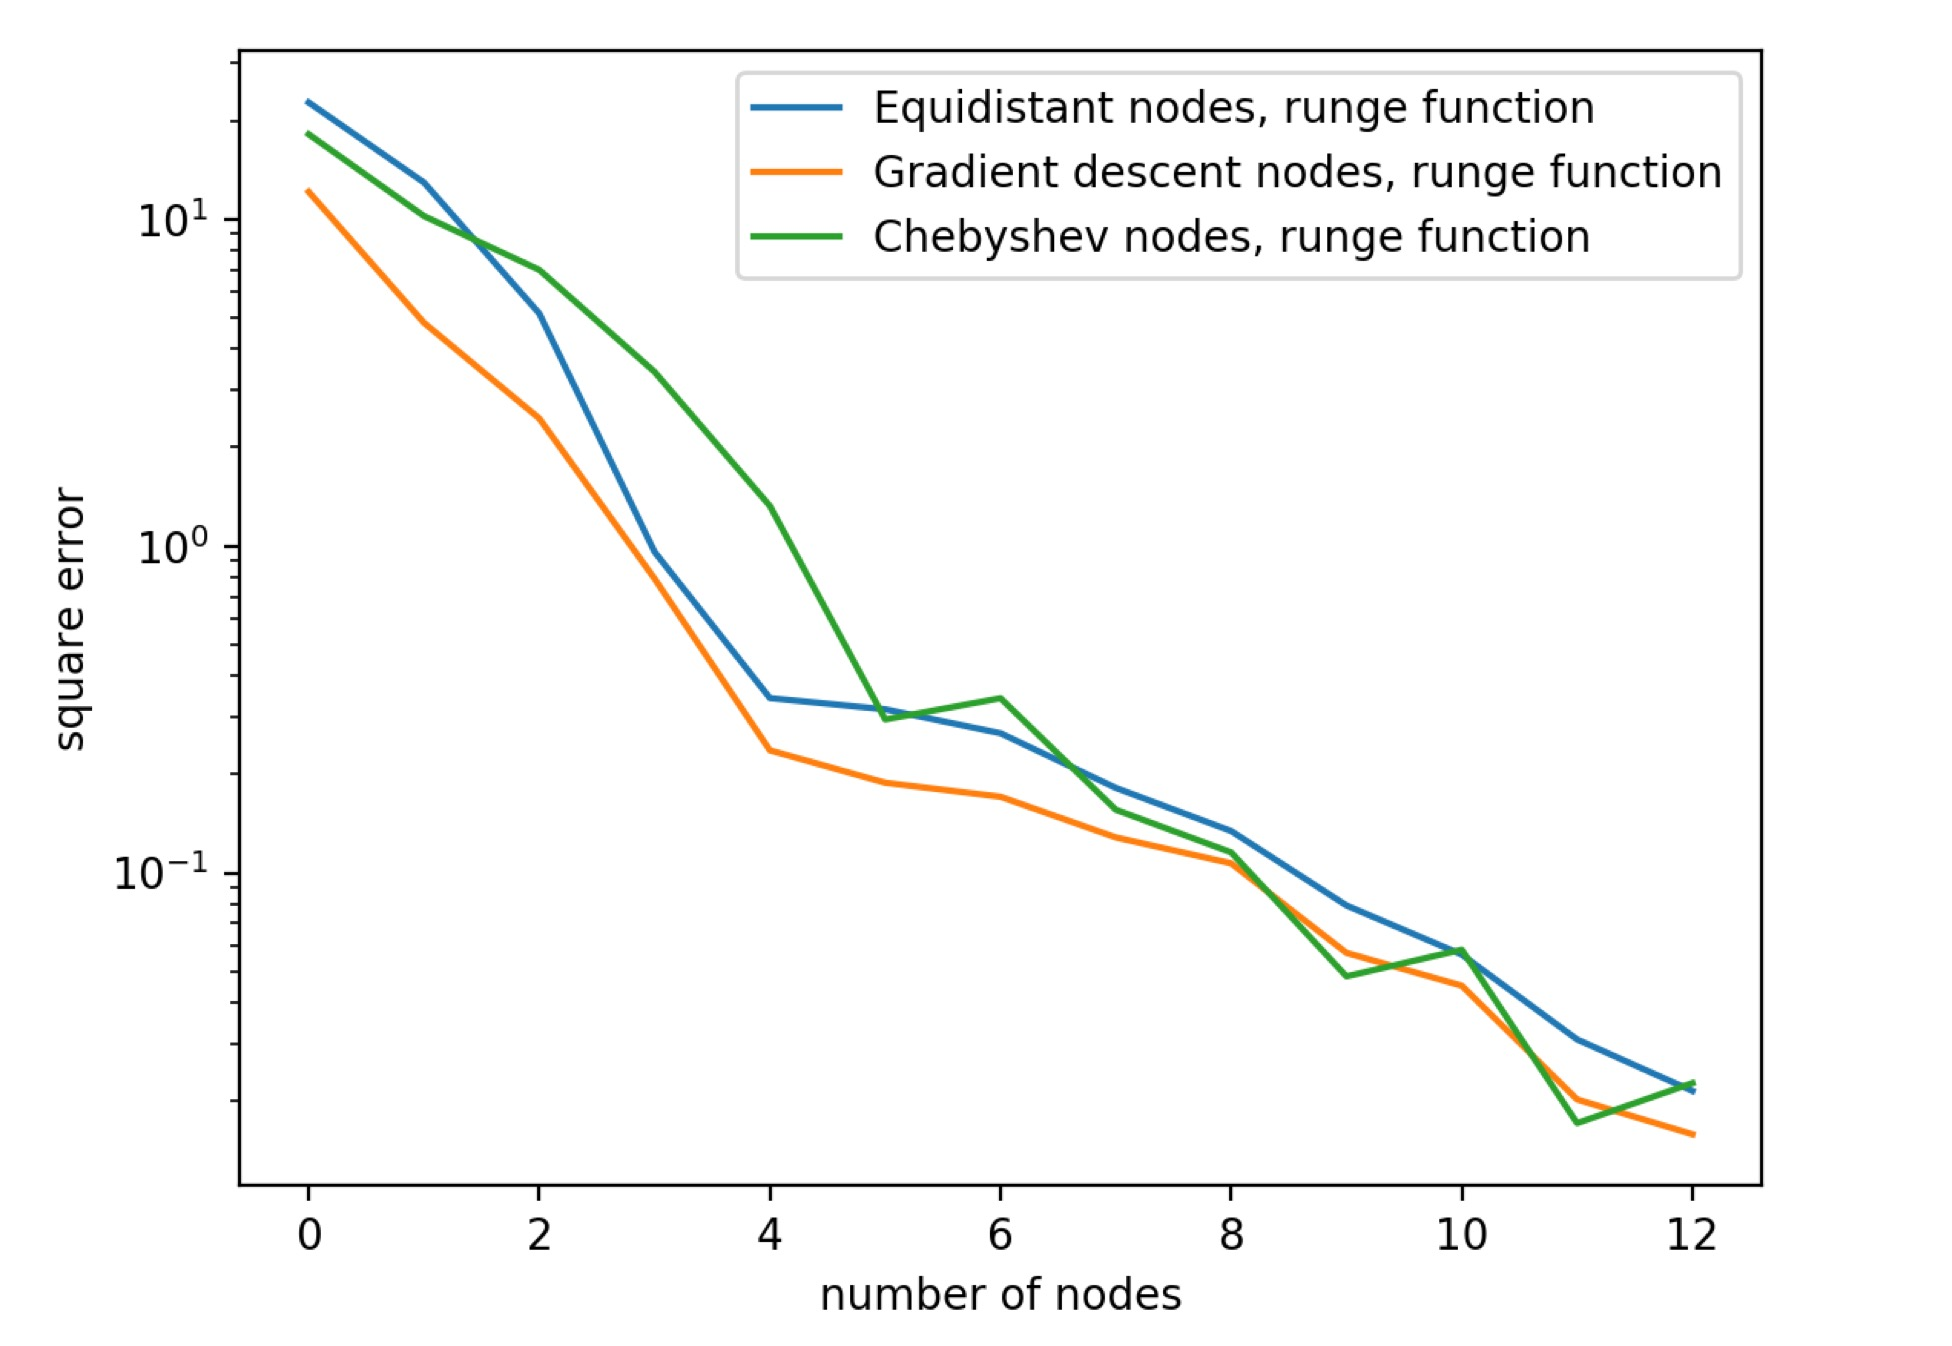
\includegraphics[width=1.05\textwidth]{vaar2020/numerical_methods/error_vs_nodes_runge_GradD} % first figure itself
        \caption{Runge}
    \end{minipage}\hfill
    \begin{minipage}{0.45\textwidth}
        \centering
        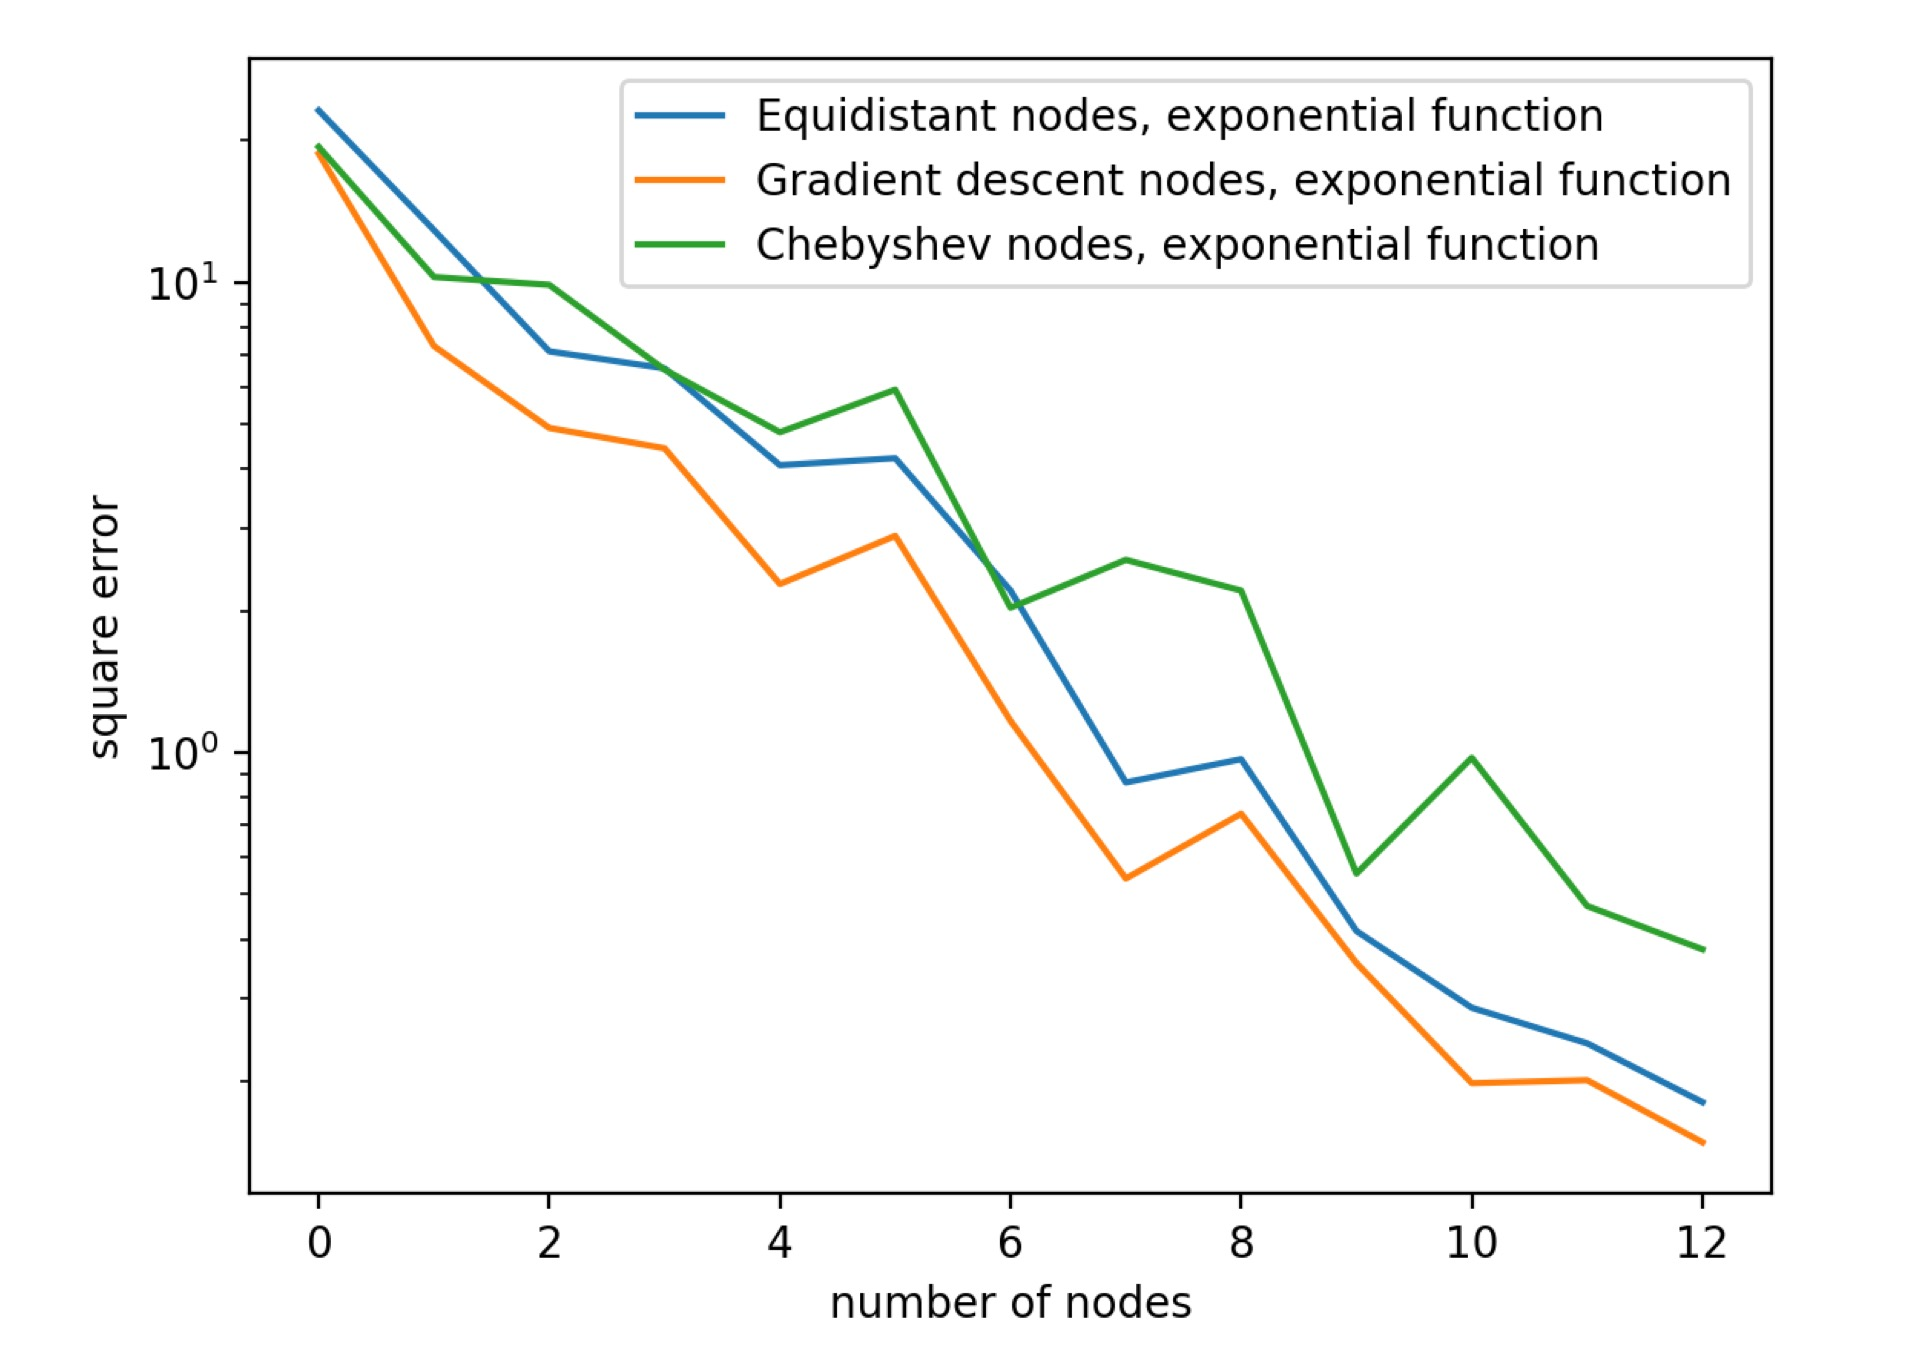
\includegraphics[width=1.05\textwidth]{vaar2020/numerical_methods/error_vs_nodes_radfunc} % second figure itself
        \caption{$h(x)$}
    \end{minipage}
\end{figure}
In these plots, I have used only $40$ iterations in the outer loop and $20$ in the inner loop, furthering the tendency that equidistant nodes are bad initial guesses for RBF on these two functions. The plots of cost versus iterations suggests that the result could have been even better with a higher number of iterations. The parameters are the same as in d), but the shape parameter e is 3.0 after discussions with fellow students. This performed better than the other values attempted, where some values even resulted in a singular matrix, which interrupted the experiment. However, this could be due to some error in the code or perhaps poor implementation.

\begin{thebibliography}{9}
  \bibitem Endre Suli & David Mayers. An Introduction to Numerical Analysis. Cambridge University Press, 2003.\label{NumAnal}
\end{thebibliography}
